\documentclass[10pt]{article}
\usepackage[margin=.7in]{geometry}\usepackage{amsmath,amssymb,tikz,hyperref}
\setlength{\parindent}{0pt}\setlength{\parskip}{5pt}
\begin{document}
\textbf{Prime-field word coefficient update}\hfill2026-10-31\\T-1149. Producer proof packet; independent source-fidelity review pending.
\section*{Checked update and hypotheses}
The word output remains canonical and decodes to
\[o+c\binom{k}{j}a^jb^{k-j}s^{-1}.\]
Hypotheses: prime $1<p<2^{31}$; canonical input words $o,c,a,b,s,i_w$; $0\le j\le k\le5$; $s\ne0$; and the checkable word certificate
\[ (s\cdot i_w)\bmod p=1.\]
Bounded multiplication decoding proves that the certificate supplies the field inverse. This verifies the supplied word, not the inversion generator.
\begin{center}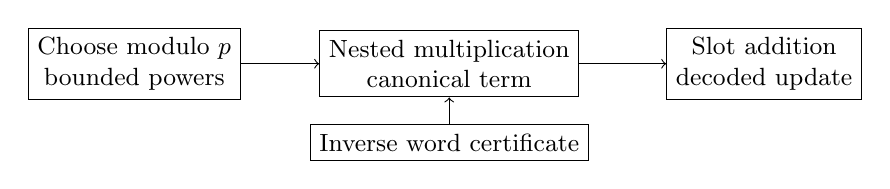
\begin{tikzpicture}[every node/.style={draw,align=center,font=\small}]
\node (a) at (0,0) {Choose modulo $p$\\bounded powers};
\node (b) at (4,0) {Nested multiplication\\canonical term};
\node (c) at (8,0) {Slot addition\\decoded update};
\node (d) at (4,-1) {Inverse word certificate};
\draw[->](a)--(b);\draw[->](b)--(c);\draw[->](d)--(b);
\end{tikzpicture}\end{center}
\section*{Supporting proofs and controls}
The source-style binary power loop unrolls symbolically for exponents zero through five; three shifts drain the exponent. Bounded choose-word reduction preserves its residue-class value. Multiplication follows the source parenthesization; addition reuses the bounded word theorem.

Nine main declarations and seventeen controls receive separate named axiom readback. With $p=17,a=2,b=3,c=4,s=2,i_w=9,k=2,j=1$, the term is 7, agreeing with $24\bmod17$; prior slot 10 updates to 0. Controls cover zero exponent/base, $(-1)^5$, reduced choose, invalid indices and wrong/zero/noncanonical inverse certificates.

Inverse word 26 passes the product test for scale 2 modulo 17 but fails canonicality. For the excluded input $2^{63}$ times 2 modulo 5, the natural result is 1 and the UInt64 result is 0. These controls retain the input-bound distinction.
\section*{Source and evidence boundary}
The source mapping is odd-characteristic $n=1$ arithmetic without diagnostic tables. \texttt{Field::inv} rejects zero and calls \texttt{bi}; its general \texttt{modpow} uses u128 products. The arbitrary-exponent inversion generator, literal vector/compiler behavior and geometric class transport remain separate bindings. Exact excerpts and source hashes accompany this packet.

One main attempt needed an explicit import of the existing nonzero-decoding lemma. The first controls needed predicate unfolding for decidability; corrected checks passed. Native exits, unchanged bindings and axiom readback are retained with all attempts. Existing compiled dependencies remain in the trust boundary.

References: existing UInt64Residue/CrossScaling/WordAdd11 proofs and \href{https://leanprover-community.github.io/mathlib4_docs/Mathlib/Data/ZMod/Basic.html}{Mathlib ZMod.Basic}. No scientific campaign, curve enumeration, timing or cost ratio. Cohort and campaign limits unchanged. Diagram shows proof dependencies.
\end{document}
